\documentclass[
nopagebreaks,
style=klope,
fleqn]{powerdot}
\usepackage{amsmath, amsfonts}
\usepackage{hyperref}
\usepackage{breakurl}
\usepackage{paralist}
\usepackage{subfig}
\usepackage{algpseudocode}
\usepackage{algorithmicx}
\usepackage{algorithm}
\usepackage{multirow}
\title{K-Means Clustering on GPU}
\author{Yige Hu and Zhiting Zhu}
\date{}

\begin{document}

\maketitle

% declaration of the new block
\algblock{ParFor}{EndParFor}
% customizing the new block
\algnewcommand\algorithmicparfor{\textbf{parfor}}
\algnewcommand\algorithmicpardo{\textbf{do}}
\algnewcommand\algorithmicendparfor{\textbf{end\ parfor}}
\algrenewtext{ParFor}[1]{\algorithmicparfor\ #1\ \algorithmicpardo}
\algrenewtext{EndParFor}{\algorithmicendparfor}

\algnewcommand\algorithmicinput{\textbf{INPUT:}}
\algnewcommand\INPUT{\item[\algorithmicinput]}

\newcommand{\TB}[0]{threadblock\xspace}
\newcommand{\TBs}[0]{threadblocks\xspace}
\newcommand{\SM}[0]{streaming multiprocessor\xspace}
\newcommand{\SMs}[0]{streaming multiprocessors\xspace}
\newcommand{\gcc}[0]{gcc\xspace}
\newcommand{\clang}[0]{clang\xspace}
\newcommand\norm[1]{\left\lVert#1\right\rVert}
\newcommand\numberthis{\addtocounter{equation}{1}\tag{\theequation}}

\begin{slide} {Problem}
  \begin{compactitem}
  \item{Input: a set of data points $\{x_i|i = 1..n\} \subseteq
    \mathbb{R}^d $}
  \item{Task: partition the n data points
    in to k($\leq n$) sets S = $\{S_1, S_2, ..., S_k\}$ so as to minimize
    the within-cluster sum of squared
    errors, $$\arg\min_{S}\sum_{i=1}^{k}\sum_{x \in S_i} \parallel x -
    \mu(S_i)\parallel$$ where $\mu(S_i)$ is the mean of points in $S_i$}
  \item{NP-hard problem for global optimal solution
    \begin{compactitem}
    \item{In general d dimension Euclidean space even with 2 clusters~\cite{k-means-euclidean}}
    \item{k clusters in the same plane~\cite{k-means-plane}}
    \end{compactitem}
  }
  \item{Heuristic algorithm}
  \end{compactitem}
  \vspace{-0.6in}
  \begin{figure}
    \flushright
    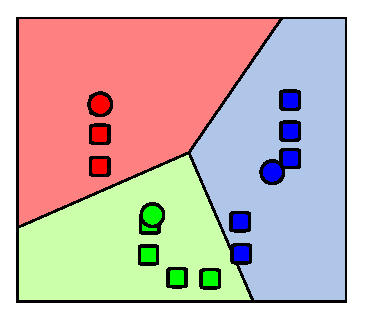
\includegraphics[scale=.5]{fig/K_Means_Example_Step_4.eps}
  \end{figure}
\end{slide}

\begin{slide} {Sequential Algorithm: Example}
  \begin{figure}[h]
    \centering
    \subfloat[t][~\cite{f1}]{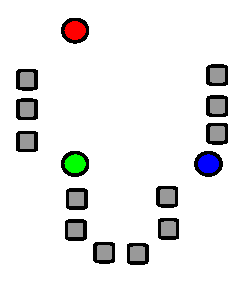
\includegraphics[scale=.5]{fig/K_Means_Example_Step_1.eps}}\qquad
    \subfloat[t][~\cite{f2}]{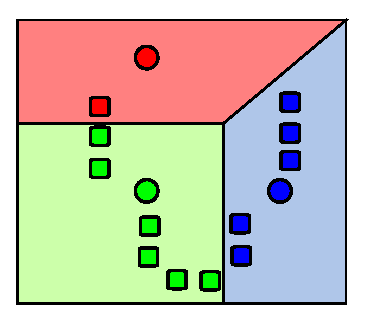
\includegraphics[scale=.5]{fig/K_Means_Example_Step_2.eps}}\\
    \subfloat[t][~\cite{f3}]{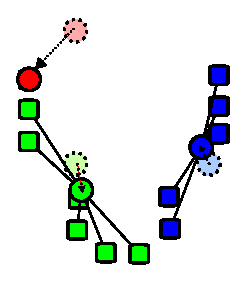
\includegraphics[scale=.5]{fig/K_Means_Example_Step_3.eps}}\qquad
    \subfloat[t][~\cite{f4}]{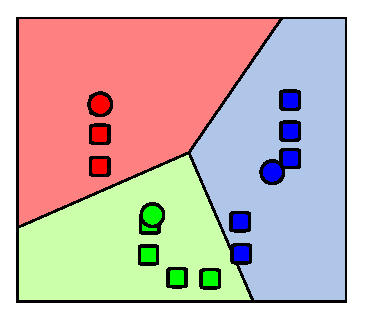
\includegraphics[scale=.5]{fig/K_Means_Example_Step_4.eps}}
  \end{figure}
  \begin{compactitem}
  \item{Problem size: $N$ $d$-dimensional data points, put into $K$ clusters.}
  \end{compactitem}
\end{slide}

\begin{slide} {Sequential Algorithm}
  \footnotesize
  \begin{algorithmic}[1]
    \INPUT $K$: Number of clusters; $N$: number of $d$-dimensional data points; $p$: data points. 
    \Function{seq\_k-means}{$p, N, K$}
    \State Randomly generate $K$ points as cluster centroids $c[]$
    \While {!termination\_condition }
    \For {i = 1..N}
    \For {j = 1..K}
    \For {dd = 1..d}
    \State $distance += (p(i)(dd) - c(j)(dd))^2$
    \EndFor
    \EndFor
    \State Find the nearest centroid $c_{nearest}$ for $p(i)$
    \State Assign each point to the nearest cluster centroid
    \State Accumulate $p(i)$'s coordinates
    \State Divide the accumulated coords by num\_points to get the new centroid
    \EndFor
    \State Recalculate termination condition
    \EndWhile
    \EndFunction
  \end{algorithmic}
  \begin{compactitem}
    \vspace{.1in}
  \item{Suppose the algorithm runs m iterations. Time complexity: O(NKdm)}
  \end{compactitem}
\end{slide}

\begin{slide} {Intuitive Parallel Algorithm}
  \footnotesize
  \begin{algorithmic}[1]
    \INPUT $K$: Number of clusters; $N$: number of d-dimensional data points; $p$: data points.
    \Function{par\_k-means}{$p, N, K$} \label{alg:p}
    \State Randomly choose $K$ points as cluster centroids $c[]$
    \While {! termination\_condition}
    \ParFor {i = 1..N}
    \For {j = 1..K}
    \For {dd = 1..d}
    \State $distance += (p(i)(dd) - c(j)(dd))^2$
    \EndFor
    \EndFor
    \State Find the nearest centroid $c_{nearest}$ for $p(i)$
    \State Change membership of $p(i)$ to the cluster with $c_{nearest}$
    \State Accumulate $p(i)$'s coordinates to the cluster's new centroid
    \EndParFor
    \State Compute new $c[]$: divide the accumulated coords by num\_points
    \State Recalculate termination condition
    \EndWhile
    \EndFunction  
  \end{algorithmic}
  \begin{compactitem}
    \vspace{5mm}
  \item{Suppose m iterations. 
    Work: O(NKdm), Depth: O(Kdm).}
  \end{compactitem}
\end{slide}

\begin{slide}{K-means with Matrix Operation}
  \footnotesize
  \begin{compactitem}
  \item{Suppose $p(i) = (p_{i1}, p_{i2}, ..., p_{id})$ and $c(j) = (c_{j1},
    c_{j2}, ..., c_{jd})$, the squared Euclidean distance between point p(i) and centroid c(j) is: 
    \begin{align}
      dist^2(p(i),c(j)) &= \norm{\vec{p_i} - \vec{c_i}}^2 \\
             &= \norm{\vec{p_i}}^2 - 2 \vec{p_i} \cdot \vec{c_i}^T + \norm{\vec{c_i}}^2 
  \end{align}}
  \item{
      $\norm{\vec{p_i}}$ and $\norm{\vec{c_i}}$ are vector norms of each row of the matrices p and c
  }
  \item{
      $\vec{p_i} \cdot \vec{c_i}^T$ is a matrix production 
  }
  \item{Computing distance between each point with each centroid can be restructured as matrix operations: norm and production}
  \end{compactitem}
\end{slide}

\begin{slide}{K-means with Matrix Operation}
  \scriptsize
  \begin{algorithmic}[1]
    \INPUT $K$: Number of clusters; $N$: number of $d$-dimensional data points; $p$: data points.
    \Function{par\_k-means-matrix}{$p, N, K$} \label{alg:pm}
    \State Randomly choose $K$ points as cluster centroids $c[]$
    \For {i = 1..N}
    \State $p\_norm\_2(i) = \norm{p(i))}^2$
    \EndFor
    \While {! termination\_condition}
    \For {j = 1..K}
    \State $c\_norm\_2(j) = \norm{(c(j))}^2$
    \EndFor
    \State $pc\_product = 2 p \cdot c^T$
    \ParFor {i = 1..N}
    \For {j = 1..K}
    \State $distance = p\_norm\_2(i) + c\_norm\_2(j) - pc\_product(i)(j)$
    \EndFor
    \State Find the nearest centroid $c_{nearest}$ for $p(i)$
    \State Change membership of $p(i)$ to the cluster with $c_{nearest}$
    \State Accumulate $p(i)$'s coordinates to the cluster's new centroid
    \EndParFor
    \State Compute new $c[]$: divide the accumulated coords by num\_points
    \State Recalculate termination condition
    \EndWhile
    \EndFunction
  \end{algorithmic}
  \vspace{.1cm}
  \tiny
  \begin{compactitem}
  \item{Work = $O(Nd + Kdm + NKdm + NKm + Ndm)$}
  \item{Depth = $O(D(norm(d))*N + (norm(d))*K*m + D(matrix product(NKd))*m + Km + dm)$}
  \end{compactitem}
\end{slide}

\begin{slide}{K-means with Matrix Operation}
  \begin{compactitem}
  \item{Implement using cuBLAS}
  \item{Matrix-matrix multiplication -- cublasSgemm}
  \item{Vector norm -- cublasSnrm2}
  \item{cublasSnrm2 is pretty slow but cublasSgemm is efficient
    \begin{compactitem}
    \item{Need to calculate vector norm of each row of matrix but no such function in cuBLAS}
    \end{compactitem}
  }
  \item{Use matrix multiplication to compute vector norm of all rows of matrix
    \begin{compactitem}
    \item{For a matrix A, the norm of each row of matrix is at the diagonal of $A * A^T$}
    \item{For example: 
      $
      \begin{bmatrix}
        a & b & c\\
        d & e & f
      \end{bmatrix}
      *
      \begin{bmatrix}
        a & d \\
        b & e \\
        c & f
      \end{bmatrix}
      =
      \begin{bmatrix}
        a^2+b^2+c^2 & ad + be + cf \\
        ad + be + cf & d^2 + e^2 + f^2
      \end{bmatrix}
      $
    }  
    \end{compactitem}
  } 
  \end{compactitem}
\end{slide}

\begin{slide}{Compute Vector Norm With Matrix Multiplication}
  \scriptsize
  \begin{algorithmic}[1]
    \INPUT $K$: Number of clusters; $N$: number of $d$-dimensional data points; $p$: data points.
    \Function{par\_k-means-matrix-v2}{$p, N, K$} \label{alg:pm2}
    \State Randomly choose $K$ points as cluster centroids $c[]$
    \State $p\_norm\_2 = diag(p * p^T)$
    \While {! termination\_condition}
    \State $c\_norm\_2 = diag(c * c^T)$
    \State $pc\_product = 2 p \cdot c^T$
    \ParFor {i = 1..N}
    \For {j = 1..K}
    \State $distance = p\_norm\_2(i) + c\_norm\_2(j) - pc\_product(i)(j)$
    \EndFor
    \State Find the nearest centroid $c_{nearest}$ for $p(i)$
    \State Change membership of $p(i)$ to the cluster with $c_{nearest}$
    \State Accumulate $p(i)$'s coordinates to the cluster's new centroid
    \EndParFor
    \State Compute new $c[]$: divide the accumulated coords by num\_points
    \State Recalculate termination condition
    \EndWhile
    \EndFunction
  \end{algorithmic}
  \vspace{.1cm}
  \begin{compactitem}
  \item{Work = $O(N^2d + K^2dm + NKdm + NKm + Ndm)$}
  \item{Depth = $O(D(matrix product(N^2d)) + D(matrix product(K^2d)*m) + D(matrix product(NKd))*m+ Km + dm)$}
  \end{compactitem}
\end{slide}

\begin{slide}{Optimization: CUDA Memory Hierachy}
  \begin{figure}[!h]
  \centering
  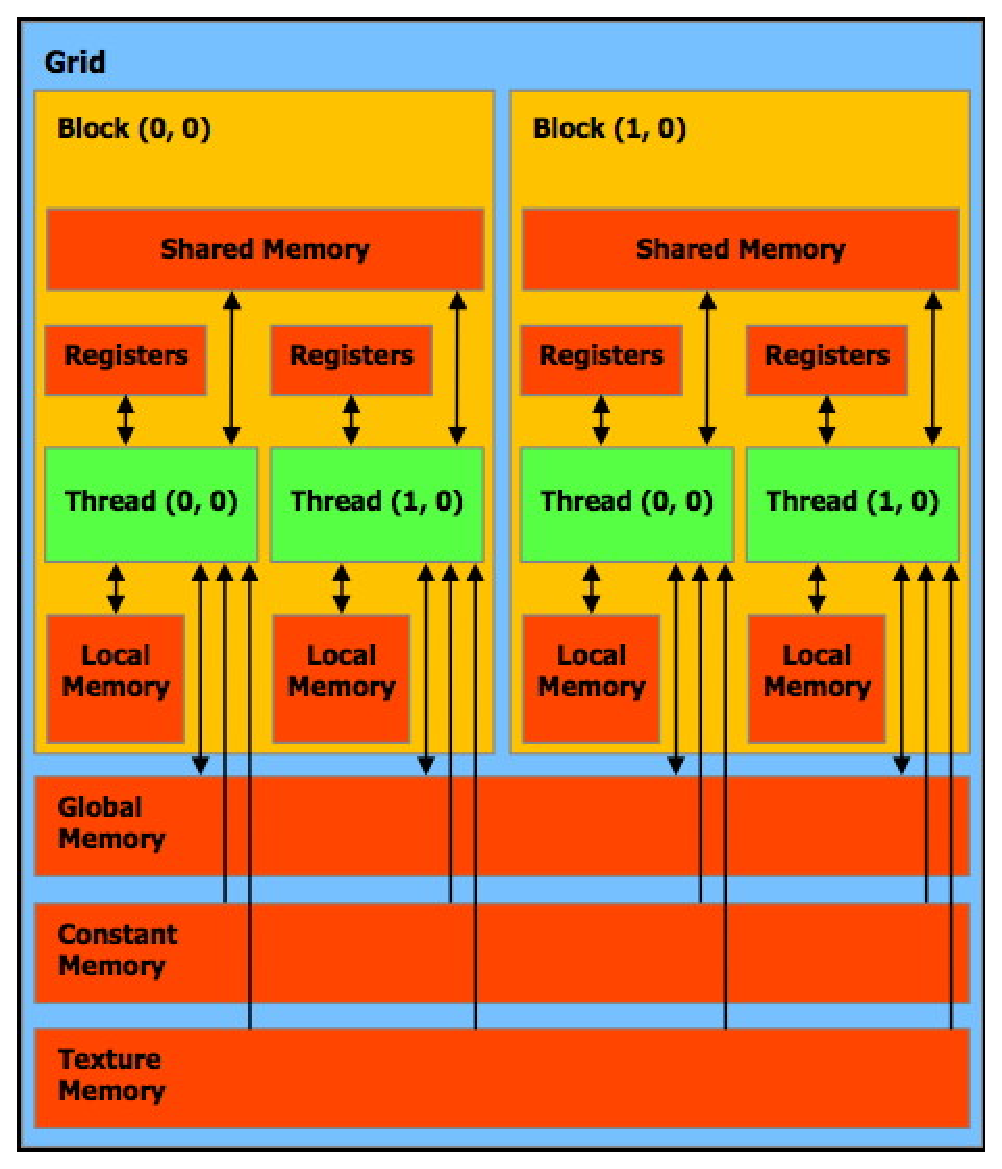
\includegraphics[height=0.6\textheight]{fig/cuda_memory}
  \caption{CUDA Memory Hierachy: global memory, shared memory, registers}
  \label{fig:cuda_memory}
  \end{figure}

\end{slide}

\begin{slide}{Optimizations}
  \begin{compactitem}
  \item{Coalesced memory access to global memory}
    \begin{figure}[!h]
    \centering
    \includegraphics[width=0.7\linewidth]{fig/access1}
    \caption{Sequential and aligned access}
    \label{fig:access1}
    \end{figure}
  \item{High-speed memory: e.g. shared memory}
  \item{Prefetching / pragma unroll}
  \end{compactitem}
\end{slide}

\begin{slide}{Evaluation Platform and Implementation}
  \small
  \begin{compactitem}
  \item{Nvidia M2090 GPU
    \begin{compactitem}
    \item{Fermi architecture, compute 2.0 capability}
    \item{CUDA 6.5 Driver, 5.0 Runtime and cuBLAS}
    \item{Nvidia driver 340.29}
    \item{16 Multiprocessors, 32 threads per wrap, 48 wraps per multiprocessor, 1536 threads per
      multiprocessor. In total, 24576 threads}
    \item{Maximum 1024 threads per block}
    \end{compactitem}
  }
  \item{Intel Xeon X5680 3.33 Hz processor}
  \item{Performance is influenced by GPU hardware and CUDA version
    \begin{compactitem}
    \item{Runs faster in a GPU with a GPU with the same architecture using CUDA 6.5}  
    \end{compactitem}
  }
  \item{Test strong and weak scaling for the first parallel algorithm}
  \item{Cannot control how many threads cuBLAS is using
    \begin{compactitem}
    \item{Compare performance among three parallel algorithms with the same input size}
    \end{compactitem}
  }
  \item{Different initial centroid assignment may lead to different number of iterations
    \begin{compactitem}
    \item{Enforce same number of iterations and same number of centroids}
    \end{compactitem}
  }
  \end{compactitem}
\end{slide}

\begin{slide}{Strong Scalability}
  \begin{compactitem}
  \item{Input size: 640000 points, 40 dimension. 120 centroids, 50 iterations}
  \item{Configuration: 1024 threads/TB}
  \end{compactitem}
  \begin{figure}[!h]
    \centering
    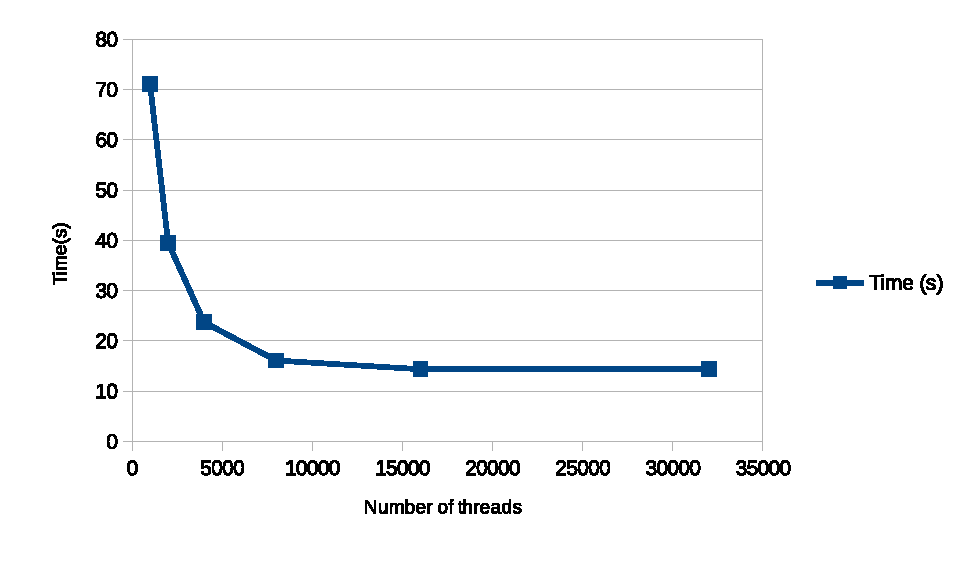
\includegraphics[width=0.7\linewidth]{fig/strong_scaling}
    \caption{Strong scaling test for the first parallel algorithm}
    \label{fig:strong_scaling}
  \end{figure}
\end{slide}

\begin{slide}{Weak Scalability}
  \begin{compactitem}
  \item{The input size is propotinal to the total number of threads}
  \item{Input: 40-dimensional points, 120 cluster centroids, 128 points/TB}
  \item{Configuration: 128 threads/TB}
  \end{compactitem}
  \begin{figure}[!h]
    \centering
    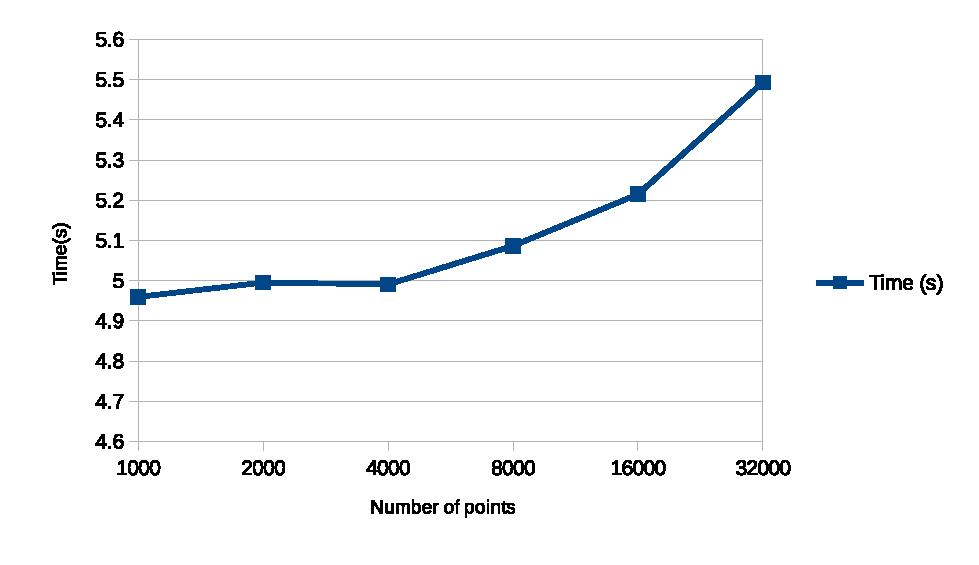
\includegraphics[width=0.7\linewidth]{fig/weak_scaling}
    \caption{Weak scaling test for the first parallel algorithm}
    \label{fig:weak_scaling}
  \end{figure}
\end{slide}

\begin{slide}{Comparison between Sequential and Three Parallel Algorithms}
  \begin{compactitem}
  \item{Each point with 40 dimension. 120 centroids and run 50 iterations}
  \item{Handle one point per thread for the first parallel algorithm}
  \item{Configuration: 1024 threads/TB}
  \end{compactitem}
  \begin{figure}[!h]
    \centering
    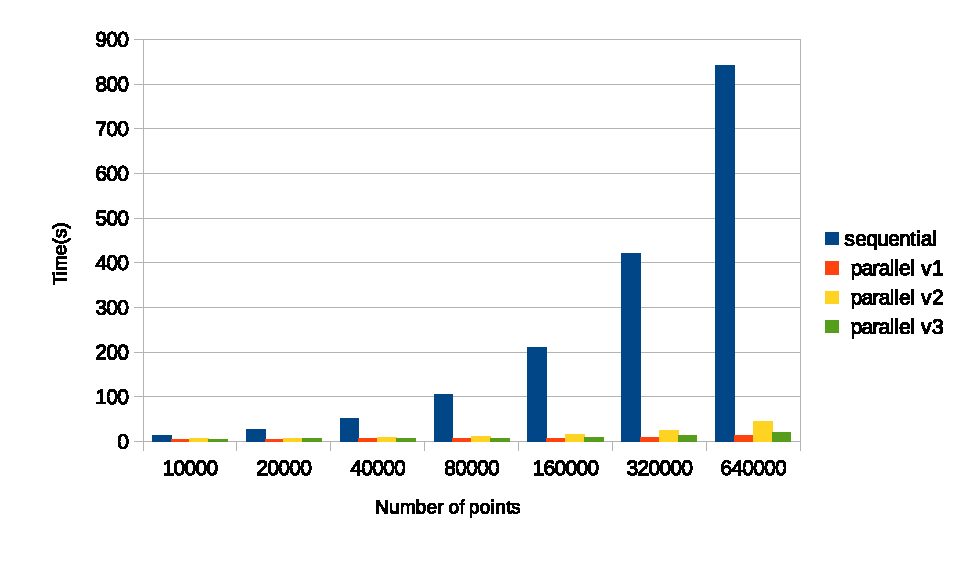
\includegraphics[width=0.7\linewidth]{fig/all_comparison}
    \caption{Comparison of running time between sequential and three versions of parallel algorithms}
    \label{fig:all}
  \end{figure}
\end{slide}

\begin{slide}{Comparison between Three Parallel Algorithms}
  \begin{figure}[!h]
    \centering  
    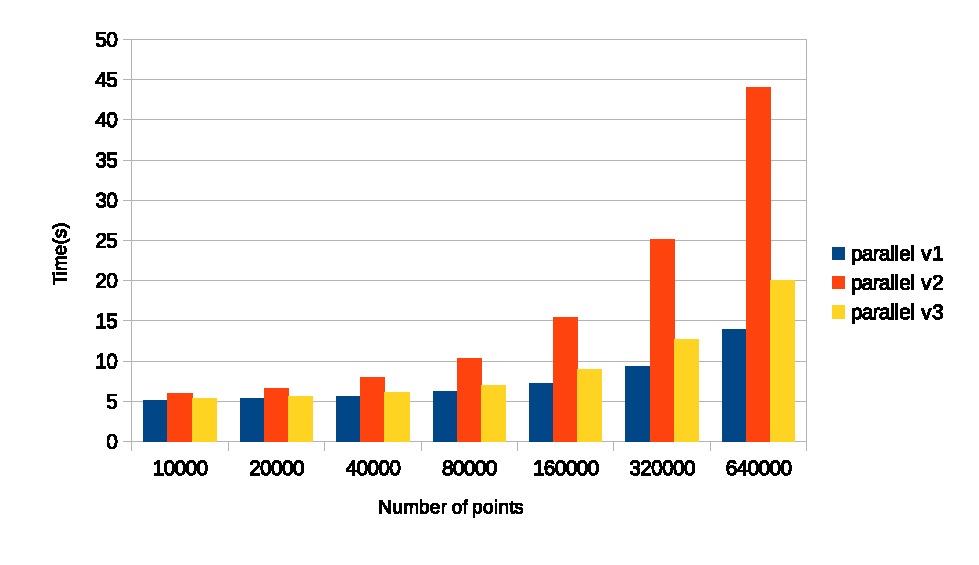
\includegraphics[width=0.9\linewidth]{fig/parallel_algorithm_comparison}
    \caption{Comparison of three parallel algorithms}
    \label{fig:par}
  \end{figure}
\end{slide}

\begin{slide} {References}
\footnotesize
\bibliographystyle{acm}
\bibliography{bibliography}
\end{slide}
\end{document}
